\section{Giới thiệu}
\subsection{Đặt vấn đề}

Trong vòng nhiều thế kỷ qua, chúng ta đã chứng kiến sự tăng vọt của lượng dữ liệu người dùng khổng lồ, tạo nền tảng tài nguyên để vận hành các thuật toán học máy và học sâu nhằm xây dựng các hệ thống hướng dữ liệu. Và nổi bật trong các hệ thống như vậy đó chính là các mô hình ngôn ngữ lớn – Large Language model (LLM), có khả năng tạo sinh dữ liệu đáng kinh ngạc đến mức mà các nhà khoa học đương thời gọi chúng là các SOTA (state of the art – tạm dịch Đỉnh cao của công nghệ). Các tác tử hoạt động dựa trên các mô hình đó cũng dần xuất hiện, trong đó, các tác tử đối thoại (conversational agents) hay gọi một cách quen thuộc hơn là các AI chatbot đã dần khẳng định được vị thế của mình trong cộng đồng ứng dụng trí tuệ nhân tạo tạo sinh.

Theo một thống kê thực tế từ đầu năm 2018 của Hubspot, số lượng hàng hóa bán ra cho người dùng trên toàn thế giới thông qua chatbot chiếm tới hơn 47\% và con số này cho đến nay chắc chắn đã lớn hơn rất nhiều. Một báo cáo khác, thực hiện bởi trang Fortune Business Insights, dự đoán thị trường chatbot sẽ tăng từ 396,2 triệu USD (năm 2019) đến 1953,3 triệu USD (năm 2027), tương ứng với tốc độ tăng trưởng CAGR đạt 22.5\%. Con số này đã phần nào chứng minh chatbot đang ngày càng được ứng dụng rộng rãi trong cuộc sống, đặc biệt là trong lĩnh vực kinh doanh. Rất nhiều doanh nghiệp kinh doanh trong lĩnh vực dịch vụ trên toàn cầu đã ưu tiên triển khai chatbot để xử lý hiệu quả tình huống khi nhu cầu khách hàng tăng cao nhưng đội ngũ nhân viên ít ỏi không đủ sức đảm đương.

\begin{figure}[!ht]
    \centering
    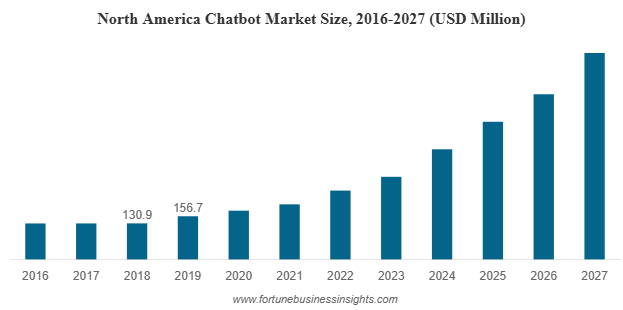
\includegraphics[width=\linewidth]{Images/P1/da2.png}
    \vspace{0.5cm}
    \caption{Thị trường chatbot ở Bắc Mỹ dự đoán đến năm 2027 (triệu USD)}
\end{figure}

Một phân tích khác trên trang web market.us cho biết, phân khúc đám mây đang chiếm giữ thị phần áp đảo so với các hệ thống chatbot on-premise (doanh nghiệp tự triển khai) – chiếm khoảng 64.7\% vào năm 2023. Sự thống lĩnh này phần lớn là nhờ tính linh hoạt, khả năng mở rộng và hiệu quả về chi phí mà các nhà cung cấp giải pháp đám mây đem lại, điều mà các doanh nghiệp rất ưa chuộng, bởi họ có thể dễ dàng mở rộng quy mô các giải pháp chatbot của mình theo nhu cầu khách hàng hiện tại mà không tốn công sức đầu tư cho các hạ tầng máy móc cần thiết. Hơn nữa, chatbot AI dựa trên đám mây được hưởng lợi từ các bản cập nhật và cải tiến liên tục do công nghệ điện toán đám mây tạo ra. Các nhà cung cấp có thể triển khai các bản cập nhật trực tiếp vào cơ sở hạ tầng đám mây, đảm bảo rằng tất cả người dùng đều được hưởng lợi từ những tiến bộ mới nhất trong AI và máy học mà không phải trả thêm chi phí hoặc nỗ lực nào. Vị thế dẫn đầu của phân khúc Đám mây cũng được củng cố bởi sự tin tưởng ngày càng tăng vào các biện pháp bảo mật đám mây và việc áp dụng ngày càng nhiều các môi trường làm việc linh động và từ xa, đòi hỏi các giải pháp linh hoạt và dễ tiếp cận.

\newpage

\begin{figure}[!ht]
    \centering
    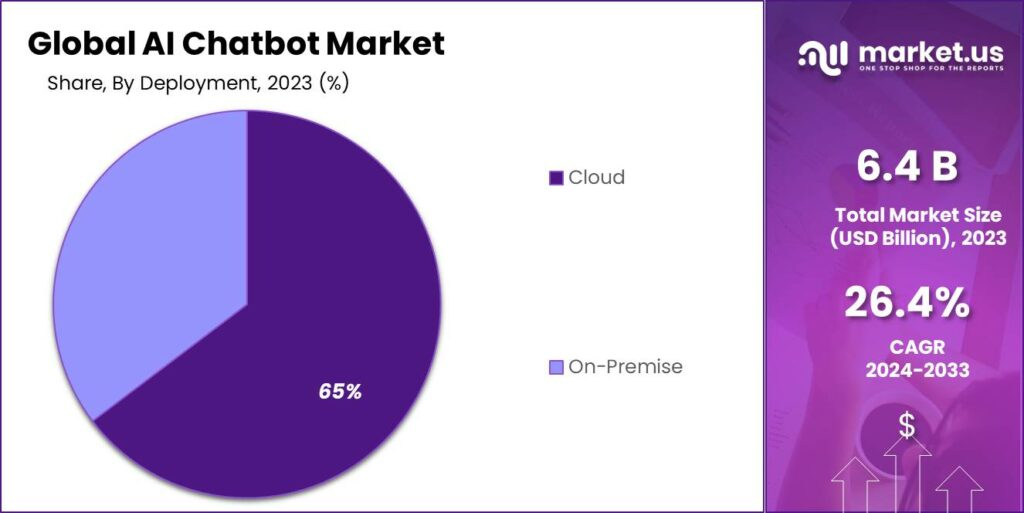
\includegraphics[width=\linewidth]{Images/P1/da3.jpg}
    \vspace{0.5cm}
    \caption{Thị phần chatbot năm 2023 phân theo nơi triển khai}
\end{figure}

Về khía cạnh chọn nền tảng để gắn chatbot vào, Website luôn là ưu tiên hàng đầu bởi chúng chính là mặt tiền kỹ thuật số của một doanh nghiệp và hình ảnh một chatbot với lô gô của doanh nghiệp ở góc dưới cùng bên phải màn hình đã trở thành một điều quen thuộc trong tiềm thức của khách hàng. Ngày nay chatbot hỗ trợ đã trở thành một người bạn đồng hành phổ biến trong hành trình trải nghiệm của người dùng khi truy cập một website thương mại điện tử của doanh nghiệp. Xu hướng này dự kiến sẽ tiếp tục khi ngày càng nhiều các công ty nhận ra tầm quan trọng của việc tăng cường sự tương tác của khách hàng trên các kênh kỹ thuật số chính của họ, khiến các tác tử đối thoại này trở thành một yêu cầu chức năng không thể thiếu khi xây dựng các trang web kinh doanh.

\begin{figure}[!ht]
    \centering
    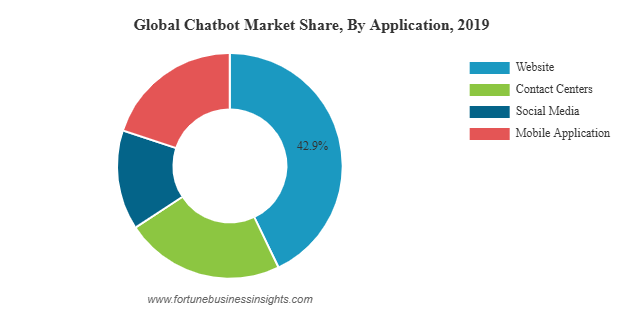
\includegraphics[width=\linewidth]{Images/P1/da1.png}
    \vspace{0.5cm}
    \caption{Thị phần các nền tảng để gắn chatbot năm 2019}
\end{figure}

Các lợi ích của một chatbot hỗ trợ khách hàng:
\begin{itemize}
    \item Tăng tương tác với khách hàng: Với khả năng hoạt động liên tục 24/7, chatbots giúp các doanh nghiệp tương tác hiệu quả với khách hàng mọi lúc mọi nơi. Chúng có thể hỗ trợ đồng thời nhiều khách hàng mà không làm giảm chất lượng dịch vụ và cung cấp phản hồi nhanh chóng đảm bảo khách hàng không phải chờ đợi lâu.
    \item Tự động hóa và tiết kiệm chi phí: Bằng cách tự động hóa các quy trình hỗ trợ, như trả lời các câu hỏi thường gặp, xử lý các yêu cầu đơn giản, doanh nghiệp có thể tiết kiệm nguồn lực đáng kể. Điều này giúp cắt giảm chi phí vận hành, giảm sự phụ thuộc vào lực lượng nhân viên lớn.
    \item Hỗ trợ đa ngôn ngữ: Chatbots có thể được lập trình để hỗ trợ nhiều ngôn ngữ khác nhau, giúp mở rộng phạm vi tương tác với khách hàng từ khắp nơi trên thế giới. Điều này giúp tối ưu hóa trải nghiệm khách hàng toàn cầu và vượt qua rào cản ngôn ngữ, mở rộng thị trường.
    \item Cá nhân hóa trải nghiệm: Với khả năng thu thập và phân tích dữ liệu, chatbot có thể cung cấp các trải nghiệm tương tác được cá nhân hóa cho từng khách hàng, từ đó cải thiện sự hài lòng và lòng trung thành của khách hàng đối với thương hiệu.
    \item Nâng khả năng nhận diện thương hiệu: Chatbots không chỉ là công cụ hỗ trợ, mà còn có thể được thiết kế để phản ánh phong cách và giá trị của thương hiệu. Việc sử dụng chatbot giúp tăng cường nhận diện thương hiệu, làm cho doanh nghiệp trở nên chuyên nghiệp và hiện đại hơn trong mắt khách hàng.
\end{itemize}

Tóm lại, các công nghệ chatbot và mô hình ngôn ngữ lớn	đang trên đà phát triển chóng mặt và việc ứng dụng chúng vào một lĩnh vực cụ thể đó là chăm sóc khách hàng giúp gia tăng lợi ích kinh tế, thăng hạng trang web trong mắt người dùng và tăng cường uy tín của doanh nghiệp trong mắt những khách hàng mới. Nhu cầu phát triển một nền tảng xây dựng chatbot đám mây để phục vụ nhu cầu của doanh nghiệp trở nên bức thiết hơn bao giờ hết, giúp giảm tải khối lượng công việc cho các phòng ban IT của các công ty cũng như chi phí đầu tư cho các hệ thống on-premise.

\subsection{Các hướng giải quyết liên quan}

Với sự gia tăng nhu cầu về dịch vụ hỗ trợ 24/7 và yêu cầu về trải nghiệm cá nhân hóa, các doanh nghiệp cần bổ sung các giải pháp về các chatbot trí tuệ nhân tạo để nâng cao chất lượng dịch vụ khách hàng mà không tốn kém quá nhiều nguồn lực. Chính vì thế, đề tài của nhóm tác giả mong muốn cung cấp dịch vụ tạo chatbot nhằm giúp các doanh nghiệp:

\begin{itemize}
    \item Tiết kiệm thời gian và chi phí: Chatbots tự động hóa các quy trình cơ bản, giúp giảm thiểu chi phí nhân sự và thời gian xử lý yêu cầu.
    \item Cải thiện trải nghiệm khách hàng: Chatbots phản hồi gần như ngay lập tức và cá nhân hóa các tương tác, tạo ấn tượng tốt hơn với khách hàng, qua đó nâng cao tỷ lệ giữ chân khách hàng (Customer Retention Rate – CRR)  
    \item Tăng cường tính cạnh tranh: Trong thị trường cạnh tranh cao, việc áp dụng công nghệ tiên tiến như chatbot giúp doanh nghiệp nổi bật và dễ dàng tiếp cận với khách hàng hơn. Bên cạnh đó, chatbot cũng mang trong mình nhận diện thương hiệu, giúp ghi điểm trong mắt khách hàng qua đó tăng lợi thế cạnh tranh của công ty.
    \item Đón đầu xu hướng: Như đã đề cập, chatbots đang dần trở thành xu hướng toàn cầu, giúp doanh nghiệp không chỉ tối ưu hóa dịch vụ mà còn đi trước đối thủ trong việc áp dụng công nghệ vào quy trình kinh doanh. Công ty hòa nhập trong xu hướng chuyển đổi số của nhà nước, qua đó được tạo điều kiện thuận lơi hơn trên thương trường, mở rộng phạm vi tiếp cận khách hàng.
\end{itemize}

Cụ thể, đề tài hướng đến xây dựng một trang web cung cấp dịch vụ có đăng ký (subscription), cùng giải pháp xây dựng chatbot đám mây hỗ trợ doanh nghiệp nhiều tính năng phổ biến mà không tốn quá nhiều công sức của đội ngũ công nghệ thông tin của công ty hoặc bỏ ra chi phí để xây dựng hạ tầng phần cứng rắc rối. Khi sử dụng ứng dụng này, doanh nghiệp có thể:

\begin{itemize}
    \item Lựa chọn tài liệu phù hợp để huấn luyện chatbot, định dạng text, docs hoặc pdf đều khả dụng
    \item Tùy chỉnh logo, ảnh đại diện, màu sắc, định dạng khung chat nhằm tăng độ nhận diện thương hiệu 
    \item Đội ngũ công nghệ của công ty có thể dễ dàng tích hợp vào app, website của công ty thông qua CDN
    \item Chatbot sẽ được prompting và fine-tuning để tránh việc đưa ra các câu trả lời không phù hợp với tiêu chuẩn đạo đức
    \item Không cần trả thêm bất kỳ khoản chi phí nào khác
\end{itemize}

Đề tài sẽ tập trung vào khả năng tự động hóa các tác vụ hỗ trợ khách hàng, chẳng hạn như trả lời các câu hỏi thường gặp (FAQs), hỗ trợ mua hàng, và xử lý các vấn đề cơ bản và cuối cùng là phân tích sơ lược và thử nghiệm trong một số lĩnh vực thực tế như bán lẻ, dịch vụ để kiểm định tính hiệu quả trong các bối cảnh kinh doanh khác nhau hoặc trong giáo dục, nghiên cứu nhằm kiểm tra tính khả thi về mặt liên ngành. Nhóm tác giả mong muốn kết quả của đề tài này sẽ đóng góp vào việc nghiên cứu và phát triển các ứng dụng liên quan đến AI tạo sinh (Generative AI) cũng như liên quan đến xử lý ngôn ngữ tự nhiên (Natural language processing), từ đó mở rộng hiểu biết của chúng ta về cách thức áp dụng các mô hình ngôn ngữ lớn như một công cụ hiệu quả để tối ưu các tác vụ hỗ trợ người dùng mà cụ thể ở đây là chăm sóc khách hàng.